% answers.tex —— 2020 年·全国Ⅲ卷·理科 · 参考答案与详细解析片段
% 由 tools/generate_projects.py 依来源总账自 2020/2020_数学真题_全国3理_试题.md + 2020/2020_数学真题_全国3理_解析正文.md + 2020/2020_数学真题_全国3理_答案要点.md 生成，勿手改（改源 MD 后重跑）


\begin{answer}
\gksolhead{1}{}

\textbf{题目}：

已知集合 $A=\{(x,y)\mid x,y\in\mathbf N^*,\ y\geqslant x\}$，$B=\{(x,y)\mid x+y=8\}$，则 $A\cap B$ 中元素的个数为\mbox{（　　）}

（A）$2$；（B）$3$；（C）$4$；（D）$6$。

\Needspace{4\baselineskip}
\textbf{解析}

\Needspace{5\baselineskip}
$x$，$y$ 都是正整数，且 $y\geqslant x$。与 $x+y=8$ 联立得
\nopagebreak[4]
\[2x\leqslant x+y=8\ \Longrightarrow\ x\leqslant4 .\]
\Needspace{5\baselineskip}
于是 $x$ 只能取 $1$，$2$，$3$，$4$，对应 $y=7$，$6$，$5$，$4$，四组都满足 $y\geqslant x$，即
\nopagebreak[4]
\[A\cap B=\{(1,7),\ (2,6),\ (3,5),\ (4,4)\},\]
共 $4$ 个元素。

选 C。

\gkanswer{答案：C。由 $y\geqslant x$、$x+y=8$ 得 $x\leqslant4$，正整数解为 $(1,7)$，$(2,6)$，$(3,5)$，$(4,4)$，共 $4$ 个。}

\end{answer}
\begin{answer}
\gksolhead{2}{}

\textbf{题目}：

复数 $\dfrac1{1-3\mathrm i}$ 的虚部是\mbox{（　　）}

（A）$-\dfrac3{10}$；（B）$-\dfrac1{10}$；（C）$\dfrac1{10}$；（D）$\dfrac3{10}$。

\Needspace{4\baselineskip}
\textbf{解析}

\Needspace{5\baselineskip}
对分母实数化：
\nopagebreak[4]
\[\frac1{1-3\mathrm i}=\frac{1+3\mathrm i}{(1-3\mathrm i)(1+3\mathrm i)}=\frac{1+3\mathrm i}{1+9}=\frac1{10}+\frac3{10}\mathrm i .\]
故实部为 $\dfrac1{10}$，虚部为 $\dfrac3{10}$。

选 D。

\gkanswer{答案：D。$\dfrac1{1-3\mathrm i}=\dfrac{1+3\mathrm i}{10}=\dfrac1{10}+\dfrac3{10}\mathrm i$，虚部为 $\dfrac3{10}$。}

\end{answer}
\begin{answer}
\gksolhead{3}{}

\textbf{题目}：

在一组样本数据中，$1$，$2$，$3$，$4$ 出现的频率分别为 $p_1$，$p_2$，$p_3$，$p_4$，且 $\sum\limits_{i=1}^4p_i=1$，则下面四种情形中，对应样本的标准差最大的一组是\mbox{（　　）}

（A）$p_1=p_4=0.1$，$p_2=p_3=0.4$；（B）$p_1=p_4=0.4$，$p_2=p_3=0.1$；（C）$p_1=p_4=0.2$，$p_2=p_3=0.3$；（D）$p_1=p_4=0.3$，$p_2=p_3=0.2$。

\Needspace{4\baselineskip}
\textbf{解析}

\Needspace{5\baselineskip}
四个选项都满足 $p_1=p_4$，$p_2=p_3$。记 $p_1=p_4=a$，$p_2=p_3=b$，则
\nopagebreak[4]
\[2a+2b=1\ \Longrightarrow\ a+b=\frac12 .\]
\Needspace{5\baselineskip}
样本均值
\nopagebreak[4]
\[\bar x=1\cdot a+2\cdot b+3\cdot b+4\cdot a=5(a+b)=\frac52,\]
\Needspace{5\baselineskip}
与 $a$ 的取值无关。二阶矩
\nopagebreak[4]
\[E(X^2)=1^2\cdot a+2^2\cdot b+3^2\cdot b+4^2\cdot a=17a+13b,\]
\Needspace{5\baselineskip}
故方差
\nopagebreak[4]
\[s^2=17a+13b-\frac{25}4=17a+13\left(\frac12-a\right)-\frac{25}4=4a+\frac14 .\]
标准差随 $a$ 增大而增大。四个选项的 $a$ 依次为 $0.1$，$0.4$，$0.2$，$0.3$，故（B）的方差最大（$s^2=1.85$），标准差也最大。

选 B。

\gkanswer{答案：B。均值恒为 $\dfrac52$，方差为 $4a+\dfrac14$（$a=p_1=p_4$），（B）中 $a=0.4$ 使方差最大。}

\end{answer}
\begin{answer}
\gksolhead{4}{}

\textbf{题目}：

Logistic 模型是常用数学模型之一，可应用于流行病学领域。有学者根据公布数据建立了某地区新冠肺炎累计确诊病例数 $I(t)$（$t$ 的单位：天）的 Logistic 模型：$I(t)=\dfrac K{1+\mathrm e^{-0.23(t-53)}}$，其中 $K$ 为最大确诊病例数。当 $I(t^*)=0.95K$ 时，标志着已初步遏制疫情，则 $t^*$ 约为（$\ln19\approx3$）\mbox{（　　）}

（A）$60$；（B）$63$；（C）$66$；（D）$69$。

\Needspace{4\baselineskip}
\textbf{解析}

\Needspace{5\baselineskip}
由 $I(t^*)=0.95K$ 得
\nopagebreak[4]
\[\frac K{1+\mathrm e^{-0.23(t^*-53)}}=0.95K\ \Longrightarrow\ 1+\mathrm e^{-0.23(t^*-53)}=\frac1{0.95}=\frac{20}{19},\]
\Needspace{5\baselineskip}
故
\nopagebreak[4]
\[\mathrm e^{-0.23(t^*-53)}=\frac1{19}\ \Longrightarrow\ -0.23(t^*-53)=-\ln19 .\]
\Needspace{5\baselineskip}
于是
\nopagebreak[4]
\[t^*=53+\frac{\ln19}{0.23}\approx53+\frac3{0.23}=53+13.04=66.04,\]
故 $t^*$ 约为 $66$（若取 $\ln19\approx2.944$，得 $t^*\approx65.8$，仍约为 $66$）。

选 C。

\gkanswer{答案：C。由 $\mathrm e^{-0.23(t^*-53)}=\dfrac1{19}$ 得 $t^*=53+\dfrac{\ln19}{0.23}\approx53+13=66$。}

\end{answer}
\begin{answer}
\gksolhead{5}{}

\textbf{题目}：

设 $O$ 为坐标原点，直线 $x=2$ 与抛物线 $C:y^2=2px$（$p>0$）交于 $D$，$E$ 两点。若 $OD\perp OE$，则 $C$ 的焦点坐标为\mbox{（　　）}

（A）$\left(\dfrac14,0\right)$；（B）$\left(\dfrac12,0\right)$；（C）$(1,0)$；（D）$(2,0)$。

\Needspace{4\baselineskip}
\textbf{解析}

\Needspace{5\baselineskip}
在 $x=2$ 上，$y^2=2p\cdot2=4p$，故可设
\nopagebreak[4]
\[D(2,\ 2\sqrt p),\qquad E(2,\ -2\sqrt p).\]
\Needspace{5\baselineskip}
则
\nopagebreak[4]
\[\overrightarrow{OD}\cdot\overrightarrow{OE}=2\times2+2\sqrt p\times(-2\sqrt p)=4-4p .\]
\Needspace{5\baselineskip}
由 $OD\perp OE$ 得 $4-4p=0$，即 $p=1$。此时 $C:y^2=2x$，焦点为
\nopagebreak[4]
\[\left(\frac p2,0\right)=\left(\frac12,0\right).\]

选 B。

\gkanswer{答案：B。$D(2,2\sqrt p)$，$E(2,-2\sqrt p)$，$\overrightarrow{OD}\cdot\overrightarrow{OE}=4-4p=0$ 得 $p=1$，焦点为 $\left(\dfrac12,0\right)$。}

\end{answer}
\begin{answer}
\gksolhead{6}{}

\textbf{题目}：

已知向量 $\boldsymbol a$，$\boldsymbol b$ 满足 $|\boldsymbol a|=5$，$|\boldsymbol b|=6$，$\boldsymbol a\cdot\boldsymbol b=-6$，则 $\cos\langle\boldsymbol a,\boldsymbol a+\boldsymbol b\rangle=$\mbox{（　　）}

（A）$-\dfrac{31}{35}$；（B）$-\dfrac{19}{35}$；（C）$\dfrac{17}{35}$；（D）$\dfrac{19}{35}$。

\Needspace{4\baselineskip}
\textbf{解析}

\Needspace{5\baselineskip}
先算
\nopagebreak[4]
\[\boldsymbol a\cdot(\boldsymbol a+\boldsymbol b)=|\boldsymbol a|^2+\boldsymbol a\cdot\boldsymbol b=25-6=19 .\]
\Needspace{5\baselineskip}
再算
\nopagebreak[4]
\[|\boldsymbol a+\boldsymbol b|^2=|\boldsymbol a|^2+2\boldsymbol a\cdot\boldsymbol b+|\boldsymbol b|^2=25-12+36=49,\]
\Needspace{5\baselineskip}
故 $|\boldsymbol a+\boldsymbol b|=7$。于是
\nopagebreak[4]
\[\cos\langle\boldsymbol a,\boldsymbol a+\boldsymbol b\rangle=\frac{\boldsymbol a\cdot(\boldsymbol a+\boldsymbol b)}{|\boldsymbol a|\,|\boldsymbol a+\boldsymbol b|}=\frac{19}{5\times7}=\frac{19}{35} .\]

选 D。

\gkanswer{答案：D。$\boldsymbol a\cdot(\boldsymbol a+\boldsymbol b)=25-6=19$，$|\boldsymbol a+\boldsymbol b|=\sqrt{25+36-12}=7$，故 $\cos\langle\boldsymbol a,\boldsymbol a+\boldsymbol b\rangle=\dfrac{19}{35}$。}

\end{answer}
\begin{answer}
\gksolhead{7}{}

\textbf{题目}：

在 $\triangle ABC$ 中，$\cos C=\dfrac23$，$AC=4$，$BC=3$，则 $\cos B=$\mbox{（　　）}

（A）$\dfrac19$；（B）$\dfrac13$；（C）$\dfrac12$；（D）$\dfrac23$。

\Needspace{4\baselineskip}
\textbf{解析}

\Needspace{5\baselineskip}
在 $\triangle ABC$ 中，$AC=4$，$BC=3$，$\cos C=\dfrac23$。由余弦定理
\nopagebreak[4]
\[AB^2=AC^2+BC^2-2\cdot AC\cdot BC\cdot\cos C=16+9-2\times4\times3\times\frac23=25-16=9,\]
\Needspace{5\baselineskip}
故 $AB=3$。再由余弦定理
\nopagebreak[4]
\[\cos B=\frac{AB^2+BC^2-AC^2}{2\cdot AB\cdot BC}=\frac{9+9-16}{2\times3\times3}=\frac2{18}=\frac19 .\]

选 A。

\gkanswer{答案：A。$AB^2=16+9-2\times4\times3\times\dfrac23=9$，$AB=3$，故 $\cos B=\dfrac{9+9-16}{2\times3\times3}=\dfrac19$。}

\end{answer}
\begin{answer}
\gksolhead{8}{}

\textbf{题目}：

下图为某几何体的三视图，则该几何体的表面积是\mbox{（　　）}

（A）$6+4\sqrt2$；（B）$4+4\sqrt2$；（C）$6+2\sqrt3$；（D）$4+2\sqrt3$。
\nopagebreak[4]
\begin{center}% 2020 全国Ⅲ卷 理8：某几何体的三视图
% 来源 PDF：普通高考/2020/2020全国3理(云南,广西,贵州,西藏,四川).pdf 第 1 页（A3 横排），印面 1125，第 8 题题干下方
% 结构（按原页矢量数据换算）：主视图、左视图、俯视图均为腰长 2 的等腰直角三角形；
%   主视图直角在右下，左视图直角在左下，俯视图直角在右上。三视图的直角互相对应，
%   故该几何体是三条两两垂直的棱长均为 2 的四面体。
% 尺寸标注：原页只在主视图底边、主视图右边、俯视图右边标出「2」，此处照录。
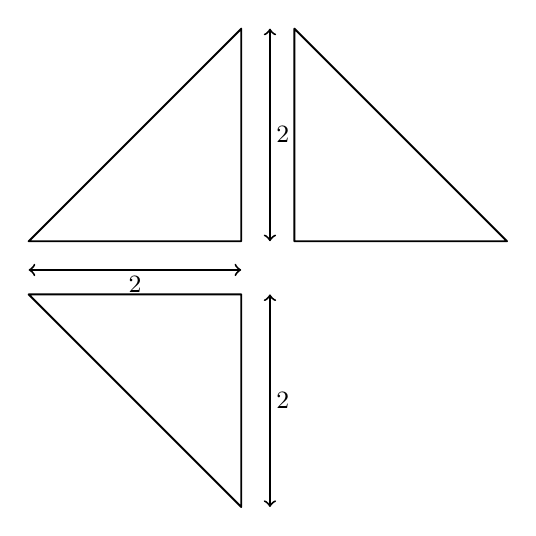
\begin{tikzpicture}[line width=0.7pt, font=\small,
  x=1.35cm, y=1.35cm, line cap=round, line join=round]

  % 主视图：直角边 2 与 2，直角在右下
  \draw (0,0) -- (2,0) -- (2,2) -- cycle;

  % 左视图：直角边 2 与 2，直角在左下
  \draw (2.5,0) -- (4.5,0) -- (2.5,2) -- cycle;

  % 俯视图：直角边 2 与 2，直角在右上
  \draw (0,-0.5) -- (2,-0.5) -- (2,-2.5) -- cycle;

  % 尺寸标注
  \draw[<->] (0,-0.27) -- (2,-0.27) node[midway, below, inner sep=2pt] {$2$};
  \draw[<->] (2.27,0) -- (2.27,2) node[midway, right, inner sep=2pt] {$2$};
  \draw[<->] (2.27,-0.5) -- (2.27,-2.5) node[midway, right, inner sep=2pt] {$2$};
\end{tikzpicture}
\end{center}
\nopagebreak[4]
\Needspace{4\baselineskip}
\textbf{解析}

三视图都是腰长为 $2$ 的等腰直角三角形：俯视图说明底面是直角边长 $2$ 的等腰直角三角形；主视图、左视图的竖直边长均为 $2$，说明过底面直角顶点有一条长为 $2$ 的棱垂直于底面。因此该几何体是三条两两垂直、长度均为 $2$ 的棱所构成的四面体（正方体的一角）。

\Needspace{5\baselineskip}
其中三个面都是直角边长 $2$ 的直角三角形，面积各为
\nopagebreak[4]
\[\frac12\times2\times2=2,\]
\Needspace{5\baselineskip}
三面合计 $6$。第四个面的三边都是边长为 $2$ 的正方形的对角线，即
\nopagebreak[4]
\[\sqrt{2^2+2^2}=2\sqrt2,\]
\Needspace{5\baselineskip}
它是边长 $2\sqrt2$ 的正三角形，面积为
\nopagebreak[4]
\[\frac{\sqrt3}4\times(2\sqrt2)^2=\frac{\sqrt3}4\times8=2\sqrt3 .\]
\Needspace{5\baselineskip}
所以表面积为
\nopagebreak[4]
\[6+2\sqrt3 .\]

选 C。

\gkanswer{答案：C。三视图对应三条两两垂直的棱长均为 $2$ 的四面体，三个直角面面积各为 $2$，第四个面是边长 $2\sqrt2$ 的正三角形、面积 $2\sqrt3$，故表面积为 $6+2\sqrt3$。}

\end{answer}
\begin{answer}
\gksolhead{9}{}

\textbf{题目}：

已知 $2\tan\theta-\tan\left(\theta+\dfrac\pi4\right)=7$，则 $\tan\theta=$\mbox{（　　）}

（A）$-2$；（B）$-1$；（C）$1$；（D）$2$。

\Needspace{4\baselineskip}
\textbf{解析}

\Needspace{5\baselineskip}
记 $t=\tan\theta$。由和角公式
\nopagebreak[4]
\[\tan\left(\theta+\frac\pi4\right)=\frac{\tan\theta+1}{1-\tan\theta}=\frac{t+1}{1-t},\]
\Needspace{5\baselineskip}
条件化为
\nopagebreak[4]
\[2t-\frac{t+1}{1-t}=7 .\]
\Needspace{5\baselineskip}
两边同乘 $1-t$（由 $t\neq1$）：
\nopagebreak[4]
\[2t(1-t)-(t+1)=7(1-t),\]
\Needspace{5\baselineskip}
整理得
\nopagebreak[4]
\[-2t^2+t-1=7-7t\ \Longrightarrow\ -2t^2+8t-8=0\ \Longrightarrow\ t^2-4t+4=0,\]
即 $(t-2)^2=0$，故 $t=2$。

选 D。

\gkanswer{答案：D。令 $t=\tan\theta$，条件化为 $2t-\dfrac{t+1}{1-t}=7$，即 $(t-2)^2=0$，故 $t=2$。}

\end{answer}
\begin{answer}
\gksolhead{10}{}

\textbf{题目}：

若直线 $l$ 与曲线 $y=\sqrt x$ 和 $x^2+y^2=\dfrac15$ 都相切，则 $l$ 的方程为\mbox{（　　）}

（A）$y=2x+1$；（B）$y=2x+\dfrac12$；（C）$y=\dfrac12x+1$；（D）$y=\dfrac12x+\dfrac12$。

\Needspace{4\baselineskip}
\textbf{解析}

\Needspace{5\baselineskip}
设 $l$ 与 $y=\sqrt x$ 相切于点 $(a,\sqrt a)$（$a>0$）。由 $y'=\dfrac1{2\sqrt x}$，切线斜率为 $\dfrac1{2\sqrt a}$，切线方程为
\nopagebreak[4]
\[y=\sqrt a+\frac{x-a}{2\sqrt a}=\frac{x}{2\sqrt a}+\frac{\sqrt a}2,\]
\Needspace{5\baselineskip}
即
\nopagebreak[4]
\[x-2\sqrt a\,y+a=0 .\]
\Needspace{5\baselineskip}
$l$ 与圆 $x^2+y^2=\dfrac15$ 相切，故原点到 $l$ 的距离等于半径 $\dfrac1{\sqrt5}$：
\nopagebreak[4]
\[\frac{a}{\sqrt{1+4a}}=\frac1{\sqrt5}\ \Longrightarrow\ 5a^2=1+4a\ \Longrightarrow\ 5a^2-4a-1=0,\]
\Needspace{5\baselineskip}
解得 $a=1$（$a>0$，另一根 $-\dfrac15$ 舍去）。代回得
\nopagebreak[4]
\[l:\ y=\frac12x+\frac12 .\]
检验：圆心到 $x-2y+1=0$ 的距离为 $\dfrac{1}{\sqrt5}$，恰等于半径；而 $y=\dfrac12x+\dfrac12$ 与 $y=\sqrt x$ 联立得 $x-2\sqrt x+1=0$，即 $(\sqrt x-1)^2=0$，在 $x=1$ 处相切。

选 D。

\gkanswer{答案：D。设切点 $(a,\sqrt a)$，切线为 $y=\dfrac{x}{2\sqrt a}+\dfrac{\sqrt a}2$，由到原点距离 $\dfrac{a}{\sqrt{4a+1}}=\dfrac1{\sqrt5}$ 得 $a=1$，故 $l:y=\dfrac12x+\dfrac12$。}

\end{answer}
\begin{answer}
\gksolhead{11}{}

\textbf{题目}：

设双曲线 $C:\dfrac{x^2}{a^2}-\dfrac{y^2}{b^2}=1$（$a>0$，$b>0$）的左、右焦点分别为 $F_1$，$F_2$，离心率为 $\sqrt5$。$P$ 是 $C$ 上一点，且 $F_1P\perp F_2P$。若 $\triangle PF_1F_2$ 的面积为 $4$，则 $a=$\mbox{（　　）}

（A）$1$；（B）$2$；（C）$4$；（D）$8$。

\Needspace{4\baselineskip}
\textbf{解析}

\Needspace{5\baselineskip}
记 $|PF_1|=m$，$|PF_2|=n$。由 $PF_1\perp PF_2$，
\nopagebreak[4]
\[m^2+n^2=|F_1F_2|^2=(2c)^2=4c^2 .\]
\Needspace{5\baselineskip}
又
\nopagebreak[4]
\[S_{\triangle PF_1F_2}=\frac12mn=4\ \Longrightarrow\ mn=8 .\]
\Needspace{5\baselineskip}
由双曲线定义 $|m-n|=2a$，两边平方：
\nopagebreak[4]
\[4a^2=(m-n)^2=m^2+n^2-2mn=4c^2-16\ \Longrightarrow\ c^2-a^2=4,\]
\Needspace{5\baselineskip}
即 $b^2=4$。又离心率 $e=\dfrac ca=\sqrt5$，即 $c^2=5a^2$，故
\nopagebreak[4]
\[4=b^2=c^2-a^2=4a^2\ \Longrightarrow\ a^2=1\ \Longrightarrow\ a=1 .\]

选 A。

\gkanswer{答案：A。由 $PF_1\perp PF_2$ 得 $|PF_1|^2+|PF_2|^2=4c^2$，又 $|PF_1||PF_2|=8$、$\bigl||PF_1|-|PF_2|\bigr|=2a$，故 $c^2-a^2=4$，结合 $c^2=5a^2$ 得 $a=1$。}

\end{answer}
\begin{answer}
\gksolhead{12}{}

\textbf{题目}：

已知 $5^5<8^4$，$13^4<8^5$。设 $a=\log_53$，$b=\log_85$，$c=\log_{13}8$，则\mbox{（　　）}

（A）$a<b<c$；（B）$b<a<c$；（C）$b<c<a$；（D）$c<a<b$。

\Needspace{4\baselineskip}
\textbf{解析}

\Needspace{5\baselineskip}
先证 $a<b$。由换底公式，
\nopagebreak[4]
\[a<b\iff\log_53<\log_85\iff\log_53\cdot\log_58<1 .\]
\Needspace{5\baselineskip}
注意 $3\times8=24<25=5^2$，由均值不等式
\nopagebreak[4]
\[\log_53\cdot\log_58\leqslant\left(\frac{\log_53+\log_58}2\right)^2=\left(\frac{\log_524}2\right)^2<\left(\frac{\log_525}2\right)^2=1,\]
故 $a<b$。

\Needspace{5\baselineskip}
再定 $b$ 与 $c$ 的位置。由 $5^5<8^4$ 得 $5<8^{4/5}$，即
\nopagebreak[4]
\[b=\log_85<\frac45 .\]
\Needspace{5\baselineskip}
由 $13^4<8^5$ 得 $13<8^{5/4}$，即 $\log_813<\dfrac54$，取倒数得
\nopagebreak[4]
\[c=\log_{13}8=\frac1{\log_813}>\frac45 .\]
\Needspace{5\baselineskip}
所以
\nopagebreak[4]
\[a<b<\frac45<c,\]
即 $a<b<c$。

选 A。

\gkanswer{答案：A。由 $\log_53\cdot\log_58<1$ 得 $a<b$；由 $5^5<8^4$ 得 $b<\dfrac45$，由 $13^4<8^5$ 得 $c>\dfrac45$，故 $a<b<c$。}

\end{answer}
\begin{answer}
\gksolhead{13}{}

\textbf{题目}：

若 $x$，$y$ 满足约束条件 $\begin{cases}x+y\geqslant0,\\2x-y\geqslant0,\\x\leqslant1,\end{cases}$ 则 $z=3x+2y$ 的最大值为\gkblank{}。

\Needspace{4\baselineskip}
\textbf{解析}

\Needspace{5\baselineskip}
约束条件对应三条边界直线 $x+y=0$，$2x-y=0$，$x=1$，可行域是三角形，三顶点为
\nopagebreak[4]
\[(0,0),\qquad (1,-1),\qquad (1,2).\]
\Needspace{5\baselineskip}
分别代入 $z=3x+2y$：
\nopagebreak[4]
\[z(0,0)=0,\qquad z(1,-1)=3-2=1,\qquad z(1,2)=3+4=7 .\]
故最大值为 $7$。

填 $7$。

\gkanswer{答案：$7$。可行域是顶点为 $(0,0)$，$(1,-1)$，$(1,2)$ 的三角形，$z=3x+2y$ 在 $(1,2)$ 处取最大值 $7$。}

\end{answer}
\begin{answer}
\gksolhead{14}{}

\textbf{题目}：

$\left(x^2+\dfrac2x\right)^6$ 的展开式中常数项是\gkblank{}。（用数字作答）

\Needspace{4\baselineskip}
\textbf{解析}

\Needspace{5\baselineskip}
二项展开式的通项为
\nopagebreak[4]
\[T_{k+1}=\mathrm C_6^k\left(x^2\right)^{6-k}\left(\frac2x\right)^k=\mathrm C_6^k\,2^k\,x^{12-3k}\qquad(k=0,1,\cdots,6).\]
\Needspace{5\baselineskip}
令 $x$ 的指数为零：
\nopagebreak[4]
\[12-3k=0\ \Longrightarrow\ k=4 .\]
\Needspace{5\baselineskip}
故常数项为
\nopagebreak[4]
\[\mathrm C_6^4\cdot2^4=15\times16=240 .\]

填 $240$。

\gkanswer{答案：$240$。通项 $\mathrm C_6^k2^kx^{12-3k}$ 中令 $12-3k=0$ 得 $k=4$，常数项为 $\mathrm C_6^4\cdot2^4=240$。}

\end{answer}
\begin{answer}
\gksolhead{15}{}

\textbf{题目}：

已知圆锥的底面半径为 $1$，母线长为 $3$，则该圆锥内半径最大的球的体积为\gkblank{}。

\Needspace{4\baselineskip}
\textbf{解析}

\Needspace{5\baselineskip}
圆锥的高
\nopagebreak[4]
\[h=\sqrt{3^2-1^2}=\sqrt8=2\sqrt2 .\]
\Needspace{5\baselineskip}
过轴的截面是底边长为 $2$、腰长为 $3$ 的等腰三角形，内切于圆锥的球在该截面上的截线正是这个三角形的内切圆，故球半径
\nopagebreak[4]
\[\rho=\frac{S}{p}=\frac{\frac12\times2\times2\sqrt2}{\frac{2+3+3}2}=\frac{2\sqrt2}{4}=\frac{\sqrt2}2 .\]
\Needspace{5\baselineskip}
球体积
\nopagebreak[4]
\[V=\frac43\pi\rho^3=\frac43\pi\left(\frac{\sqrt2}2\right)^3=\frac43\pi\cdot\frac{2\sqrt2}8=\frac{\sqrt2}3\pi .\]

填 $\dfrac{\sqrt2}3\pi$。

\gkanswer{答案：$\dfrac{\sqrt2}3\pi$。圆锥高 $2\sqrt2$，轴截面内切圆半径 $\rho=\dfrac{1\times2\sqrt2}{1+3}=\dfrac{\sqrt2}2$，体积 $\dfrac43\pi\rho^3=\dfrac{\sqrt2}3\pi$。}

\end{answer}
\begin{answer}
\gksolhead{16}{}

\textbf{题目}：

关于函数 $f(x)=\sin x+\dfrac1{\sin x}$ 有如下四个命题：

① $f(x)$ 的图象关于 $y$ 轴对称；

② $f(x)$ 的图象关于原点对称；

③ $f(x)$ 的图象关于直线 $x=\dfrac\pi2$ 对称；

④ $f(x)$ 的最小值为 $2$。

其中所有真命题的序号是\gkblank{}。

\Needspace{4\baselineskip}
\textbf{解析}

$f(x)=\sin x+\dfrac1{\sin x}$ 的定义域为 $\{x\mid\sin x\neq0\}$，关于原点对称。

\Needspace{5\baselineskip}
① ②：由
\nopagebreak[4]
\[f(-x)=\sin(-x)+\frac1{\sin(-x)}=-\sin x-\frac1{\sin x}=-f(x),\]
$f$ 是奇函数，图象关于原点对称，故 ② 真、① 假。

\Needspace{5\baselineskip}
③：由 $\sin(\pi-x)=\sin x$ 得
\nopagebreak[4]
\[f(\pi-x)=\sin x+\frac1{\sin x}=f(x),\]
图象关于直线 $x=\dfrac\pi2$ 对称，故 ③ 真。

④：当 $\sin x<0$ 时，$f(x)=\sin x+\dfrac1{\sin x}\leqslant-2$，且当 $\sin x\to0^-$ 时 $f(x)\to-\infty$，故 $f$ 没有最小值，④ 假。

所以真命题的序号是 ②③。

填 ②③。

\gkanswer{答案：②③。$f$ 为奇函数，图象关于原点对称；又 $f(\pi-x)=f(x)$，图象关于直线 $x=\dfrac\pi2$ 对称；而 $\sin x<0$ 时 $f(x)$ 无下界，①④ 均假。}

\end{answer}
\begin{answer}
\gksolhead{17}{}

\textbf{题目}：

设数列 $\{a_n\}$ 满足 $a_1=3$，$a_{n+1}=3a_n-4n$。

（1） 计算 $a_2$，$a_3$，猜想 $\{a_n\}$ 的通项公式并加以证明；

（2） 求数列 $\{2^na_n\}$ 的前 $n$ 项和 $S_n$。

\Needspace{4\baselineskip}
\textbf{解析}

\gksubpart{（1）}

\Needspace{5\baselineskip}
由递推式
\nopagebreak[4]
\[a_2=3a_1-4\times1=9-4=5,\qquad a_3=3a_2-4\times2=15-8=7 .\]
\Needspace{5\baselineskip}
观察 $a_1=3$，$a_2=5$，$a_3=7$，猜想
\nopagebreak[4]
\[a_n=2n+1 .\]
\Needspace{5\baselineskip}
用数学归纳法证明。$n=1$ 时 $a_1=3=2\times1+1$，成立。设 $n=k$ 时 $a_k=2k+1$，则
\nopagebreak[4]
\[a_{k+1}=3a_k-4k=3(2k+1)-4k=6k+3-4k=2k+3=2(k+1)+1,\]
\Needspace{5\baselineskip}
即 $n=k+1$ 时也成立。故对一切 $n\in\mathbf N^*$，
\nopagebreak[4]
\[a_n=2n+1 .\]

\gksubpart{（2）}

\Needspace{5\baselineskip}
由（1）得 $2^na_n=(2n+1)2^n$，故
\nopagebreak[4]
\[S_n=3\times2+5\times2^2+7\times2^3+\cdots+(2n+1)2^n. \tag{1}\]
\Needspace{5\baselineskip}
两边乘 $2$：
\nopagebreak[4]
\[2S_n=3\times2^2+5\times2^3+\cdots+(2n-1)2^n+(2n+1)2^{n+1}. \tag{2}\]
\Needspace{5\baselineskip}
$(1)-(2)$，同次幂相减，并注意 $2^2+2^3+\cdots+2^n=2^{n+1}-4$：
\nopagebreak[4]
\[\begin{aligned}
-S_n&=6+2\left(2^2+2^3+\cdots+2^n\right)-(2n+1)2^{n+1}\\
&=6+2\left(2^{n+1}-4\right)-(2n+1)2^{n+1}\\
&=2^{n+2}-2-(2n+1)2^{n+1}\\
&=(1-2n)2^{n+1}-2,
\end{aligned}\]
\Needspace{5\baselineskip}
于是
\nopagebreak[4]
\[S_n=(2n-1)2^{n+1}+2 .\]
检验：$n=1$ 时右端为 $1\times4+2=6=2a_1$；$n=2$ 时右端为 $3\times8+2=26=2a_1+4a_2$，均相符。

\gkanswer{答案（1）：$a_2=5$，$a_3=7$，$a_n=2n+1$。由递推式算得前两项，再用数学归纳法验证 $3(2k+1)-4k=2(k+1)+1$。}

\gkanswer{答案（2）：$S_n=(2n-1)2^{n+1}+2$。错位相减求和，或以 $n=1,2,3$ 验证。}

\end{answer}
\begin{answer}
\gksolhead{18}{}

\textbf{题目}：

某学生兴趣小组随机调查了某市 $100$ 天中每天的空气质量等级和当天到某公园锻炼的人次，整理数据得到下表（单位：天）：

\begin{center}
\begin{tabular}{cccc}
\toprule
空气质量等级／锻炼人次 & $[0,200]$ & $(200,400]$ & $(400,600]$ \\
\midrule
$1$（优） & $2$ & $16$ & $25$ \\
$2$（良） & $5$ & $10$ & $12$ \\
$3$（轻度污染） & $6$ & $7$ & $8$ \\
$4$（中度污染） & $7$ & $2$ & $0$ \\
\bottomrule
\end{tabular}
\end{center}

（1） 分别估计该市一天的空气质量等级为 $1$，$2$，$3$，$4$ 的概率；

（2） 求一天中到该公园锻炼的平均人次的估计值（同一组中的数据用该组区间的中点值为代表）；

（3） 若某天的空气质量等级为 $1$ 或 $2$，则称这天“空气质量好”；若某天的空气质量等级为 $3$ 或 $4$，则称这天“空气质量不好”。根据所给数据，完成下面的 $2\times2$ 列联表，并根据列联表，判断是否有 $95\%$ 的把握认为一天中到该公园锻炼的人次与该市当天的空气质量有关？

\begin{center}
\begin{tabular}{ccc}
\toprule
 & 人次 $\leqslant400$ & 人次 $>400$ \\
\midrule
空气质量好 &  &  \\
空气质量不好 &  &  \\
\bottomrule
\end{tabular}
\end{center}

\Needspace{10\baselineskip}
附：$K^2=\dfrac{n(ad-bc)^2}{(a+b)(c+d)(a+c)(b+d)}$，

\begin{center}
\begin{tabular}{cccc}
\toprule
$P(K^2\geqslant k)$ & $0.050$ & $0.010$ & $0.001$ \\
\midrule
$k$ & $3.841$ & $6.635$ & $10.828$ \\
\bottomrule
\end{tabular}
\end{center}

\Needspace{4\baselineskip}
\textbf{解析}

\gksubpart{（1）}

\Needspace{5\baselineskip}
四个等级的天数分别为
\nopagebreak[4]
\[2+16+25=43,\qquad 5+10+12=27,\qquad 6+7+8=21,\qquad 7+2+0=9,\]
\Needspace{5\baselineskip}
合计 $43+27+21+9=100$。以频率估计概率，得
\nopagebreak[4]
\[P_1=0.43,\qquad P_2=0.27,\qquad P_3=0.21,\qquad P_4=0.09 .\]

\gksubpart{（2）}

\Needspace{5\baselineskip}
三个人次区间的天数分别为
\nopagebreak[4]
\[\begin{aligned}
[0,200]&:\ 2+5+6+7=20,\qquad (200,400]:\ 16+10+7+2=35,\\
(400,600]&:\ 25+12+8+0=45 .
\end{aligned}\]
\Needspace{5\baselineskip}
各组取中点 $100$，$300$，$500$，得平均人次的估计值
\nopagebreak[4]
\[\bar x=\frac{20\times100+35\times300+45\times500}{100}=\frac{2000+10500+22500}{100}=\frac{35000}{100}=350 .\]

\gksubpart{（3）}

按空气质量好（等级 $1$，$2$）与不好（等级 $3$，$4$）分类，并把人次按 $400$ 分界合并，得

\begin{center}
\begin{tabular}{cccc}
\toprule
 & 人次 $\leqslant400$ & 人次 $>400$ & 合计 \\
\midrule
空气质量好 & $2+16+5+10=33$ & $25+12=37$ & $70$ \\
空气质量不好 & $6+7+7+2=22$ & $8+0=8$ & $30$ \\
合计 & $55$ & $45$ & $100$ \\
\bottomrule
\end{tabular}
\end{center}

\Needspace{5\baselineskip}
于是 $a=33$，$b=37$，$c=22$，$d=8$，$n=100$，
\nopagebreak[4]
\[K^2=\frac{100(33\times8-37\times22)^2}{70\times30\times55\times45}=\frac{100\times(-550)^2}{5197500}=\frac{30250000}{5197500}\approx5.820 .\]
\Needspace{5\baselineskip}
因为
\nopagebreak[4]
\[5.820>3.841,\]
所以有 $95\%$ 的把握认为一天中到该公园锻炼的人次与该市当天的空气质量有关。

\gkanswer{答案（1）：$0.43$，$0.27$，$0.21$，$0.09$。四个等级的天数依次为 $43$，$27$，$21$，$9$，各除以 $100$。}

\gkanswer{答案（2）：$350$。$\dfrac{20\times100+35\times300+45\times500}{100}=350$。}

\gkanswer{答案（3）：$K^2\approx5.820>3.841$，有 $95\%$ 的把握认为有关（列联表见解析版）。}

\end{answer}
\begin{answer}
\gksolhead{19}{}

\textbf{题目}：

如图，在长方体 $ABCD-A_1B_1C_1D_1$ 中，点 $E$，$F$ 分别在棱 $DD_1$，$BB_1$ 上，且 $2DE=ED_1$，$BF=2FB_1$。

（1） 证明：点 $C_1$ 在平面 $AEF$ 内；

（2） 若 $AB=2$，$AD=1$，$AA_1=3$，求二面角 $A-EF-A_1$ 的正弦值。
\nopagebreak[4]
\begin{center}% 2020 全国Ⅲ卷 理19：长方体 ABCD-A1B1C1D1，E 在 DD1、F 在 BB1 上
% 来源 PDF：普通高考/2020/2020全国3理(云南,广西,贵州,西藏,四川).pdf 第 2 页（A3 横排），印面 1126，第 19 题题干下方
% 结构（按原页矢量数据换算）：ABCD 为上底面，A1B1C1D1 为下底面；A 在前右、B 在后右、
%   C 在后左、D 在前左；AD = 1 为图面横向单位，AA1 = 3 为竖向单位，AB = 2 沿 45° 方向
%   以半长画出（原页即如此，AB 与 AD 在图面上等长）。
%   E 在棱 DD1 上且 2DE = ED1（自 D 向下三分之一处），F 在棱 BB1 上且 BF = 2FB1（自 B 向下三分之二处）。
% 实线：DA、AB、BC、CD、DD1、AA1、BB1、D1A1、A1B1 以及 AE、AF、A1E、A1F；
% 虚线：CC1（被遮挡的棱）、C1D1 与 C1B1（被遮挡的底棱）以及体内线段 EF。
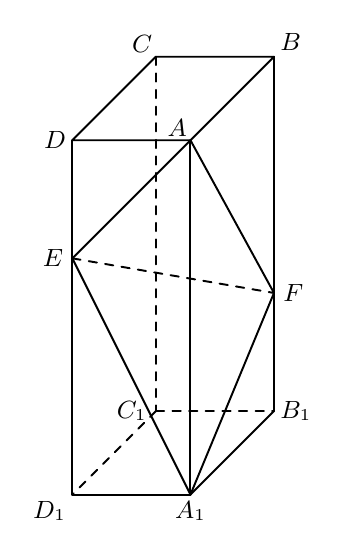
\begin{tikzpicture}[line width=0.7pt, font=\small,
  x=1.5cm, y=1.5cm, line cap=round, line join=round]

  % 顶点
  \coordinate (D)  at (0,3);
  \coordinate (A)  at (1,3);
  \coordinate (C)  at (0.70711,3.70711);
  \coordinate (B)  at (1.70711,3.70711);
  \coordinate (D1) at (0,0);
  \coordinate (A1) at (1,0);
  \coordinate (C1) at (0.70711,0.70711);
  \coordinate (B1) at (1.70711,0.70711);

  % E、F 按定比取点
  \coordinate (E) at (0,2);
  \coordinate (F) at (1.70711,1.70711);

  % 上底面
  \draw (D) -- (A) -- (B) -- (C) -- cycle;

  % 可见棱
  \draw (D) -- (D1);
  \draw (A) -- (A1);
  \draw (B) -- (B1);
  \draw (D1) -- (A1);
  \draw (A1) -- (B1);

  % 题设线段
  \draw (A) -- (E);
  \draw (A) -- (F);
  \draw (A1) -- (E);
  \draw (A1) -- (F);

  % 被遮挡的棱与体内线段
  \draw[dashed] (C) -- (C1);
  \draw[dashed] (C1) -- (D1);
  \draw[dashed] (C1) -- (B1);
  \draw[dashed] (E) -- (F);

  % 顶点标注
  \node[above left,  inner sep=1pt] at (C)  {$C$};
  \node[above right, inner sep=2pt] at (B)  {$B$};
  \node[left,        inner sep=2pt] at (D)  {$D$};
  \node[above left,  inner sep=1pt] at (A)  {$A$};
  \node[left,        inner sep=3pt] at (E)  {$E$};
  \node[right,       inner sep=3pt] at (F)  {$F$};
  \node[below left,  inner sep=2pt] at (D1) {$D_1$};
  \node[below,       inner sep=2pt] at (A1) {$A_1$};
  \node[left,        inner sep=3pt] at (C1) {$C_1$};
  \node[right,       inner sep=2pt] at (B1) {$B_1$};
\end{tikzpicture}
\end{center}
\nopagebreak[4]
\Needspace{4\baselineskip}
\textbf{解析}

\gksubpart{（1）}

\Needspace{5\baselineskip}
以 $A$ 为原点，$\overrightarrow{AB}$，$\overrightarrow{AD}$，$\overrightarrow{AA_1}$ 的方向分别为 $x$，$y$，$z$ 轴正方向建立空间直角坐标系。记 $AB=a$，$AD=b$，$AA_1=h$（$a,b,h>0$），则
\nopagebreak[4]
\[A(0,0,0),\quad B(a,0,0),\quad D(0,b,0),\quad A_1(0,0,h),\quad C_1(a,b,h).\]
\Needspace{5\baselineskip}
由 $2DE=ED_1$ 得 $DE=\dfrac13h$，故
\nopagebreak[4]
\[E\left(0,b,\frac h3\right);\]
\Needspace{5\baselineskip}
由 $BF=2FB_1$ 得 $BF=\dfrac23h$，故
\nopagebreak[4]
\[F\left(a,0,\frac{2h}3\right).\]
\Needspace{5\baselineskip}
于是
\nopagebreak[4]
\[\overrightarrow{AE}=\left(0,b,\frac h3\right),\qquad \overrightarrow{AF}=\left(a,0,\frac{2h}3\right),\]
\Needspace{5\baselineskip}
而
\nopagebreak[4]
\[\overrightarrow{AE}+\overrightarrow{AF}=\left(a,b,h\right)=\overrightarrow{AC_1},\]
即 $\overrightarrow{AC_1}$ 是平面 $AEF$ 内两个不共线向量 $\overrightarrow{AE}$，$\overrightarrow{AF}$ 的线性组合，所以 $C_1$ 在平面 $AEF$ 内。

\gksubpart{（2）}

\Needspace{5\baselineskip}
由（1）的坐标系，代入 $AB=2$，$AD=1$，$AA_1=3$ 得
\nopagebreak[4]
\[A(0,0,0),\quad E(0,1,1),\quad F(2,0,2),\quad A_1(0,0,3).\]
\Needspace{5\baselineskip}
平面 $AEF$ 的法向量可取
\nopagebreak[4]
\[\boldsymbol n_1=\overrightarrow{AE}\times\overrightarrow{AF}=(0,1,1)\times(2,0,2)=(2,2,-2)\parallel(1,1,-1).\]
\Needspace{5\baselineskip}
对平面 $A_1EF$，
\nopagebreak[4]
\[\overrightarrow{A_1E}=(0,1,-2),\qquad \overrightarrow{A_1F}=(2,0,-1),\]
\Needspace{5\baselineskip}
故其法向量可取
\nopagebreak[4]
\[\begin{aligned}
\boldsymbol n_2&=\overrightarrow{A_1E}\times\overrightarrow{A_1F}\\
&=\left(1\times(-1)-(-2)\times0,\ (-2)\times2-0\times(-1),\ 0\times0-1\times2\right)\\
&=(-1,-4,-2).
\end{aligned}\]
\Needspace{5\baselineskip}
设二面角 $A-EF-A_1$ 的大小为 $\theta$，两平面法向量的夹角为 $\varphi$，则 $\theta=\varphi$ 或 $\theta=\pi-\varphi$，故 $\sin\theta=\sin\varphi$。而
\nopagebreak[4]
\[\cos\varphi=\frac{\boldsymbol n_1\cdot\boldsymbol n_2}{|\boldsymbol n_1||\boldsymbol n_2|}=\frac{-1-4+2}{\sqrt3\cdot\sqrt{21}}=-\frac3{3\sqrt7}=-\frac1{\sqrt7},\]
\Needspace{5\baselineskip}
于是
\nopagebreak[4]
\[\sin\theta=\sin\varphi=\sqrt{1-\cos^2\varphi}=\sqrt{1-\frac17}=\sqrt{\frac67}=\frac{\sqrt{42}}7 .\]

\gkanswer{答案（1）：证明。取 $A$ 为原点建系，得 $\overrightarrow{AC_1}=\overrightarrow{AE}+\overrightarrow{AF}$，故 $C_1$ 在平面 $AEF$ 内。}

\gkanswer{答案（2）：$\dfrac{\sqrt{42}}7$。两平面法向量可取 $(1,1,-1)$ 与 $(-1,-4,-2)$，其夹角余弦为 $-\dfrac1{\sqrt7}$，故二面角的正弦值为 $\dfrac{\sqrt{42}}7$。}

\end{answer}
\begin{answer}
\gksolhead{20}{}

\textbf{题目}：

已知椭圆 $C:\dfrac{x^2}{25}+\dfrac{y^2}{m^2}=1$（$0<m<5$）的离心率为 $\dfrac{\sqrt{15}}4$，$A$，$B$ 分别为 $C$ 的左、右顶点。

（1） 求 $C$ 的方程；

（2） 若点 $P$ 在 $C$ 上，点 $Q$ 在直线 $x=6$ 上，且 $|BP|=|BQ|$，$BP\perp BQ$，求 $\triangle APQ$ 的面积。

\Needspace{4\baselineskip}
\textbf{解析}

\gksubpart{（1）}

\Needspace{5\baselineskip}
椭圆的半焦距满足 $c^2=25-m^2$，故
\nopagebreak[4]
\[e^2=\frac{c^2}{25}=\frac{25-m^2}{25}=\frac{15}{16}\ \Longrightarrow\ 25-m^2=\frac{375}{16},\]
\Needspace{5\baselineskip}
解得
\nopagebreak[4]
\[m^2=25-\frac{375}{16}=\frac{25}{16},\]
\Needspace{5\baselineskip}
所以
\nopagebreak[4]
\[C:\ \frac{x^2}{25}+\frac{y^2}{\frac{25}{16}}=1,\quad\text{\text{即}}\quad \frac{x^2}{25}+\frac{16y^2}{25}=1 .\]

\gksubpart{（2）}

\Needspace{5\baselineskip}
由（1），$C$ 即
\nopagebreak[4]
\[x^2+16y^2=25,\]
左、右顶点为 $A(-5,0)$，$B(5,0)$。

\Needspace{5\baselineskip}
设 $Q(6,q)$，则 $\overrightarrow{BQ}=(1,q)$，$|BQ|=\sqrt{1+q^2}$。由 $BP\perp BQ$ 且 $|BP|=|BQ|$，$\overrightarrow{BP}$ 由 $\overrightarrow{BQ}$ 旋转 $90^\circ$ 得到：
\nopagebreak[4]
\[\overrightarrow{BP}=(-q,1)\quad\text{\text{或}}\quad\overrightarrow{BP}=(q,-1),\]
\Needspace{5\baselineskip}
故
\nopagebreak[4]
\[P(5-q,1)\quad\text{\text{或}}\quad P(5+q,-1).\]
把 $P$ 代入 $x^2+16y^2=25$：

情形一 $P(5-q,1)$：$(5-q)^2+16=25$，即 $(5-q)^2=9$，得 $q=2$ 或 $q=8$；

情形二 $P(5+q,-1)$：$(5+q)^2+16=25$，即 $(5+q)^2=9$，得 $q=-2$ 或 $q=-8$。

\Needspace{5\baselineskip}
对 $A(-5,0)$，$P(x_P,y_P)$，$Q(6,q)$，
\nopagebreak[4]
\[S_{\triangle APQ}=\frac12\left|(x_P+5)\,q-11y_P\right| .\]
逐个代入：

$q=2$，$P(3,1)$：$S=\dfrac12|8\times2-11|=\dfrac52$；

$q=8$，$P(-3,1)$：$S=\dfrac12|2\times8-11|=\dfrac52$；

$q=-2$，$P(3,-1)$：$S=\dfrac12|8\times(-2)+11|=\dfrac52$；

$q=-8$，$P(-3,-1)$：$S=\dfrac12|2\times(-8)+11|=\dfrac52$。

\Needspace{5\baselineskip}
四种情形的面积相同，故
\nopagebreak[4]
\[S_{\triangle APQ}=\frac52 .\]

\gkanswer{答案（1）：$\dfrac{x^2}{25}+\dfrac{16y^2}{25}=1$。由 $e^2=\dfrac{25-m^2}{25}=\dfrac{15}{16}$ 得 $m^2=\dfrac{25}{16}$。}

\gkanswer{答案（2）：$\dfrac52$。设 $Q(6,q)$，由垂直且等长得 $P$ 为 $(5-q,1)$ 或 $(5+q,-1)$，代回椭圆得 $q=\pm2$ 或 $q=\pm8$，四种情形的面积同为 $\dfrac52$。}

\end{answer}
\begin{answer}
\gksolhead{21}{}

\textbf{题目}：

设函数 $f(x)=x^3+bx+c$，曲线 $y=f(x)$ 在点 $\left(\dfrac12,f\left(\dfrac12\right)\right)$ 处的切线与 $y$ 轴垂直。

（1） 求 $b$；

（2） 若 $f(x)$ 有一个绝对值不大于 $1$ 的零点，证明：$f(x)$ 所有零点的绝对值都不大于 $1$。

\Needspace{4\baselineskip}
\textbf{解析}

\gksubpart{（1）}

\nopagebreak[4]
\[f'(x)=3x^2+b .\]
\Needspace{5\baselineskip}
切线与 $y$ 轴垂直，即切线斜率为 $0$，故
\nopagebreak[4]
\[f'\left(\frac12\right)=3\times\frac14+b=\frac34+b=0\ \Longrightarrow\ b=-\frac34 .\]

\gksubpart{（2）}

\Needspace{5\baselineskip}
由（1），
\nopagebreak[4]
\[f(x)=x^3-\frac34x+c .\]
\Needspace{5\baselineskip}
设 $x_0$ 是 $f(x)$ 的一个零点且 $|x_0|\leqslant1$，则
\nopagebreak[4]
\[x_0^3-\frac34x_0+c=0\ \Longrightarrow\ c=-x_0^3+\frac34x_0 .\]
\Needspace{5\baselineskip}
于是
\nopagebreak[4]
\[f(x)=x^3-\frac34x-x_0^3+\frac34x_0=(x-x_0)\left(x^2+x_0x+x_0^2-\frac34\right).\]
\Needspace{5\baselineskip}
其余零点满足
\nopagebreak[4]
\[x^2+x_0x+x_0^2-\frac34=0 .\]
\Needspace{5\baselineskip}
其判别式
\nopagebreak[4]
\[\Delta=x_0^2-4\left(x_0^2-\frac34\right)=3-3x_0^2\geqslant0\quad(|x_0|\leqslant1),\]
\Needspace{5\baselineskip}
故另两个零点为实数
\nopagebreak[4]
\[x=\frac{-x_0\pm\sqrt{3-3x_0^2}}2,\]
\Needspace{5\baselineskip}
从而
\nopagebreak[4]
\[|x|\leqslant\frac{|x_0|+\sqrt{3-3x_0^2}}2 .\]
\Needspace{5\baselineskip}
由 $|x_0|\leqslant1$ 知 $2-|x_0|\geqslant1>0$，而
\nopagebreak[4]
\[\left(2-|x_0|\right)^2-\left(3-3x_0^2\right)=4-4|x_0|+x_0^2-3+3x_0^2=\left(2|x_0|-1\right)^2\geqslant0,\]
\Needspace{5\baselineskip}
故 $\sqrt{3-3x_0^2}\leqslant2-|x_0|$，即
\nopagebreak[4]
\[|x|\leqslant\frac{|x_0|+\left(2-|x_0|\right)}2=1 .\]
无论 $x_0=\pm1$（此时另两根相等）还是 $|x_0|<1$，都有 $|x|\leqslant1$。所以 $f(x)$ 所有零点的绝对值都不大于 $1$。

\gkanswer{答案（1）：$b=-\dfrac34$。切线与 $y$ 轴垂直给出 $f'\left(\dfrac12\right)=\dfrac34+b=0$。}

\gkanswer{答案（2）：证明。设 $|x_0|\leqslant1$ 为零点，则 $f(x)=(x-x_0)\left(x^2+x_0x+x_0^2-\dfrac34\right)$，其余零点满足 $\left|x\right|\leqslant\dfrac{|x_0|+\sqrt{3-3x_0^2}}2\leqslant1$。}

\end{answer}
\begin{answer}
\gksolhead{22}{}

\textbf{题目}【A】（选修 4—4：坐标系与参数方程）：

在直角坐标系 $xOy$ 中，曲线 $C$ 的参数方程为 $\begin{cases}x=2-t-t^2,\\y=2-3t+t^2\end{cases}$（$t$ 为参数且 $t\neq1$），$C$ 与坐标轴交于 $A$，$B$ 两点。

（1） 求 $|AB|$；

（2） 以坐标原点为极点，$x$ 轴正半轴为极轴建立极坐标系，求直线 $AB$ 的极坐标方程。

\Needspace{4\baselineskip}
\textbf{解析}

\gksubpart{（1）}

\Needspace{5\baselineskip}
令 $y=0$：
\nopagebreak[4]
\[2-3t+t^2=0\ \Longrightarrow\ t=1\ \text{\text{或}}\ t=2 .\]
由 $t\neq1$ 得 $t=2$，此时 $x=2-2-4=-4$，即 $A(-4,0)$。

\Needspace{5\baselineskip}
令 $x=0$：
\nopagebreak[4]
\[2-t-t^2=0\ \Longrightarrow\ t=1\ \text{\text{或}}\ t=-2 .\]
由 $t\neq1$ 得 $t=-2$，此时 $y=2+6+4=12$，即 $B(0,12)$。

\Needspace{5\baselineskip}
所以
\nopagebreak[4]
\[|AB|=\sqrt{(-4-0)^2+(0-12)^2}=\sqrt{16+144}=\sqrt{160}=4\sqrt{10} .\]

\gksubpart{（2）}

\Needspace{5\baselineskip}
直线 $AB$ 过 $(-4,0)$，$(0,12)$，斜率为
\nopagebreak[4]
\[k=\frac{12-0}{0-(-4)}=3,\]
\Needspace{5\baselineskip}
故其直角坐标方程为
\nopagebreak[4]
\[y=3x+12,\quad\text{\text{即}}\quad 3x-y+12=0 .\]
\Needspace{5\baselineskip}
代入 $x=\rho\cos\theta$，$y=\rho\sin\theta$，得直线 $AB$ 的极坐标方程
\nopagebreak[4]
\[3\rho\cos\theta-\rho\sin\theta+12=0,\]
\Needspace{5\baselineskip}
即
\nopagebreak[4]
\[\rho\left(\sin\theta-3\cos\theta\right)=12 .\]

\gkanswer{答案（1）：$4\sqrt{10}$。令 $y=0$ 得 $t=2$、$A(-4,0)$，令 $x=0$ 得 $t=-2$、$B(0,12)$，故 $|AB|=\sqrt{16+144}=4\sqrt{10}$。}

\gkanswer{答案（2）：$3\rho\cos\theta-\rho\sin\theta+12=0$（即 $\rho(\sin\theta-3\cos\theta)=12$）。直线 $AB$ 的直角坐标方程为 $3x-y+12=0$，代入 $x=\rho\cos\theta$，$y=\rho\sin\theta$ 即得。}

\end{answer}
\begin{answer}
\gksolhead{23}{}

\textbf{题目}【B】（选修 4—5：不等式选讲）：

设 $a$，$b$，$c\in\mathbf R$，$a+b+c=0$，$abc=1$。

（1） 证明：$ab+bc+ca<0$；

（2） 用 $\max\{a,b,c\}$ 表示 $a$，$b$，$c$ 中的最大值，证明：$\max\{a,b,c\}\geqslant\sqrt[3]4$。

\Needspace{4\baselineskip}
\textbf{解析}

\gksubpart{（1）}

\Needspace{5\baselineskip}
由 $a+b+c=0$ 得
\nopagebreak[4]
\[0=(a+b+c)^2=a^2+b^2+c^2+2(ab+bc+ca),\]
\Needspace{5\baselineskip}
故
\nopagebreak[4]
\[ab+bc+ca=-\frac{a^2+b^2+c^2}2 .\]
\Needspace{5\baselineskip}
又 $abc=1$，故 $a$，$b$，$c$ 都不为零，从而 $a^2+b^2+c^2>0$，于是
\nopagebreak[4]
\[ab+bc+ca<0 .\]

\gksubpart{（2）}

\Needspace{5\baselineskip}
设 $a=\max\{a,b,c\}$。若 $a\leqslant0$，则 $a$，$b$，$c$ 都不大于 $0$，而 $a+b+c=0$，只能 $a=b=c=0$，与 $abc=1$ 矛盾；故
\nopagebreak[4]
\[a>0 .\]
\Needspace{5\baselineskip}
由 $a+b+c=0$ 得
\nopagebreak[4]
\[b+c=-a,\]
\Needspace{5\baselineskip}
由 $abc=1$ 得
\nopagebreak[4]
\[bc=\frac1a .\]
\Needspace{5\baselineskip}
于是 $b$，$c$ 是方程
\nopagebreak[4]
\[t^2+at+\frac1a=0\]
\Needspace{5\baselineskip}
的两个实根（$t^2-(b+c)t+bc=0$ 即 $t^2+at+\dfrac1a=0$）。由判别式非负，
\nopagebreak[4]
\[a^2-\frac4a\geqslant0\ \Longrightarrow\ a^3\geqslant4\ \Longrightarrow\ a\geqslant\sqrt[3]{4},\]
\Needspace{5\baselineskip}
即
\nopagebreak[4]
\[\max\{a,b,c\}\geqslant\sqrt[3]{4} .\]

\gkanswer{答案（1）：证明。由 $(a+b+c)^2=0$ 得 $ab+bc+ca=-\dfrac{a^2+b^2+c^2}2$，而 $abc=1$ 保证 $a^2+b^2+c^2>0$，故 $ab+bc+ca<0$。}

\gkanswer{答案（2）：证明。设 $a$ 为最大值，则 $a>0$ 且 $b$，$c$ 为 $t^2+at+\dfrac1a=0$ 的两实根，判别式 $a^2-\dfrac4a\geqslant0$，故 $a^3\geqslant4$，即 $a\geqslant\sqrt[3]{4}$。}

\end{answer}